\documentclass[12pt, a4paper]{article}
%\documentclass[conference]{IEEEtran}

\title{Department of Electronic and Telecommunication Engineering}
\author{Lasitha Jananjaya\thanks{Funded by the myself.}}
\date{\today}
\usepackage{graphicx} %LaTeX package to import graphics
\graphicspath{{images/}} %configuring the graphicx package
\usepackage{amsmath}% For the equation* environment

% Language setting
% Replace `english' with e.g. `spanish' to change the document language
\usepackage[english]{babel}

% Set page size and margins
% Replace `letterpaper' with `a4paper' for UK/EU standard size
\usepackage[letterpaper,top=2cm,bottom=2cm,left=3cm,right=3cm,marginparwidth=1.75cm]{geometry}

% Useful packages
\usepackage{amsmath}
\usepackage{graphicx}
\usepackage[colorlinks=true, allcolors=blue]{hyperref}
\usepackage{ragged2e}
\usepackage{array}
\usepackage{cite}
\usepackage{wrapfig}
\usepackage{multicol}
\usepackage{float}
\usepackage{caption}

\title{Project Report Group 10}
\author{Lasitha Jananjaya}

%----------------------------------------------------------------

\begin{document}

\begin{titlepage}
   \begin{center}
       \vspace*{0.3cm}

       \begin{figure}[h]
       \centering
       
\includegraphics[width=0.45\textwidth]{University_of_Moratuwa_logo}
       %\caption{Lab project group 10}
       \label{fig:university_logo}
       \end{figure}

       \vspace*{0.2cm}

       Department of Electronic and Telecommunication Engineering

       University of Moratuwa
       \vspace{1.5cm}

       {\Large\textbf{Linear Power Supply}\par}

       \vspace{0.5cm}
       {\large{Group 29}\par}
            
       \vspace{1.5cm}

       \begin{tabular}{p{19em} l}
           \textbf{THILAKARATHNE D.L.J.} & \textbf{200650U} \\ 
           \textbf{VIKKRAMANAYAKA A.G.P.S.} & \textbf{200683X} \\  
           \textbf{VIRUTHSHAAN V.} & \textbf{200685F} \\
       \end{tabular}

       \vspace{4.5cm}
            
       This report is submitted as partial fulfillment of module
       \\EN2111 - Electronic Circuit Design
            
       \vspace{0.8cm}
       
       \today
            
   \end{center}
\end{titlepage}

%----------------------------------------------------------------

%\hline
%\newpage

%\section*{\underline{Linear Power Supply}}
%\vspace{0.2cm}
\section{Objective}

We have been tasked with the design of a linear power supply incorporating a maximum current limitation. The objective is to develop a power supply that can consistently deliver a stable output voltage, even when faced with fluctuating input line voltage conditions.

\section{Design Parameters}

\begin{itemize}
  \item Mid input voltage : 20 V
  \item Input voltage range : 18 - 22 V
  \item Mid output voltage : 12 V
  \item Output voltage range : 9 - 15 V - given
  \item Maximum output current : 100 mA
\end{itemize}

\section{Component selection and Calculations}
\subsection{Calculations}

\begin{equation}
V = \left(1+\frac{R_1}{R_2}\right)(V_Z + V_{BE})   
\end{equation}
\\
$V_Z = 4.5 V$ and $V_{BE} = 0.6 V$. Then,

\begin{equation*}
V = \left(1+\frac{R_1}{R_2}\right)(5.1)
\end{equation*}

\begin{equation}
15 < \left(1+\frac{R_x + R_v}{R_y}\right)(5.1)
\end{equation}

\begin{equation}
9 > \left(1+\frac{R_x}{R_v + R_y}\right)(5.1)
\end{equation}
\\
From 2 and 3 respectively we get,

\begin{equation*}
1.94 < \frac{R_x + R_v}{R_y}
\end{equation*}

\begin{equation*}
0.76 > \frac{R_x}{R_v + R_y}
\end{equation*}
\\
We have selected $R_v = 9.7\,k\Omega$ variable resistor.

\begin{equation}
1.94<\frac{R_z +9700}{R_y}    
\end{equation}

\begin{equation}
0.76>\frac{R_x}{9700+R_y}    
\end{equation}
\\
We have selected $ R_x = 10\,k\Omega$ variable resistor.
\begin{equation*}
1.94\,R_y < 19700 \Rightarrow R_y < 10154
\end{equation*}

\begin{equation*}
7372 + 0.76\,R_y > 10000 \Rightarrow R_y > 3458
\end{equation*}
\\
We have selected $ R_y = 10\,k\Omega$

\begin{equation}
I_{R_{min}} = \frac{V_{i_{min}} - V_{x_{max}}}{R}\,A
\end{equation}

\begin{equation*}
I_{R_{min}} = \frac{18 - 15.6}{R}\,A
\end{equation*}

\begin{equation*}
I_{R_{min}} = \frac{2.362}{R}\,A
\end{equation*}

\begin{equation}
I_{R_{min}} > \frac{I_{L_{max}}}{\beta} + I_{Z_{knee}}
\end{equation}

\begin{equation*}
10 \leq \beta < 50
\end{equation*}

\begin{equation*}
\frac{2362}{R} > \left(\frac{100}{50} + 2\right)
\end{equation*}

\begin{equation*}
\frac{2362}{4} > R
\end{equation*}

\begin{equation*}
R < 590\,\Omega
\end{equation*}

We have selected $ R = 300\,\Omega$

%\newpage
\subsection{Component selection}

\begin{itemize}
    \item Transistors \begin{itemize}
            \item BC109B : General NPN
            \item TIP31C : Power transistor
        \end{itemize}
    \item Resistors \begin{itemize}
            \item $10\,k\Omega$ - Qty 2
            \item $300\,\Omega$
            \item $5\,\Omega$
            \item Variable resistor : $10\,k\Omega$
            \item Light load : $100\,\Omega$
            \item Heavy load : $1\,k\Omega$
        \end{itemize}
\end{itemize}

%\newpage
\section{Simulation Results}

\begin{figure*}[h!]
\centering
    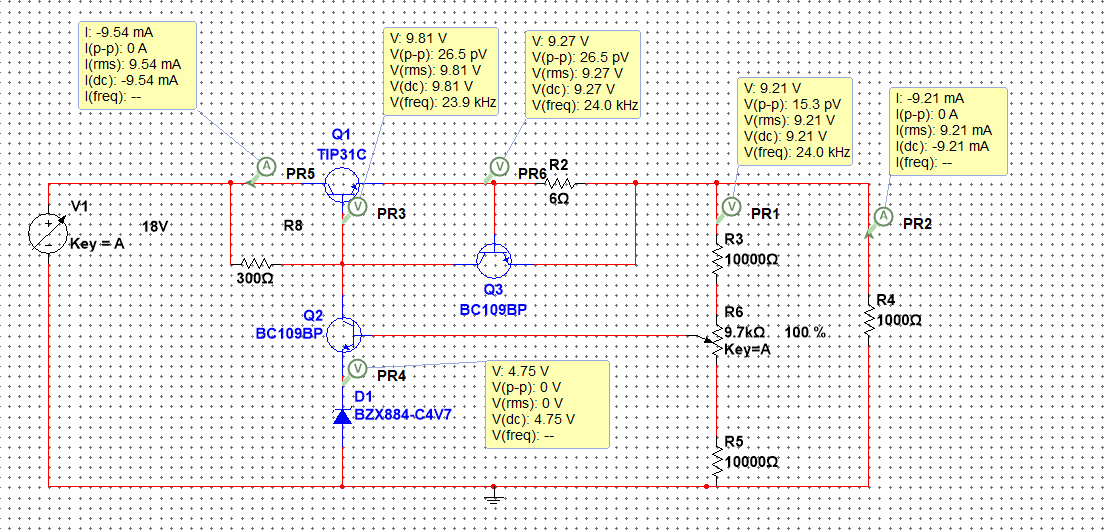
\includegraphics[width=0.7\textwidth]{lps workding.PNG}
    \caption*{Working level with $1\,k\Omega$}
\end{figure*}

\begin{figure*}[h!]
\centering
    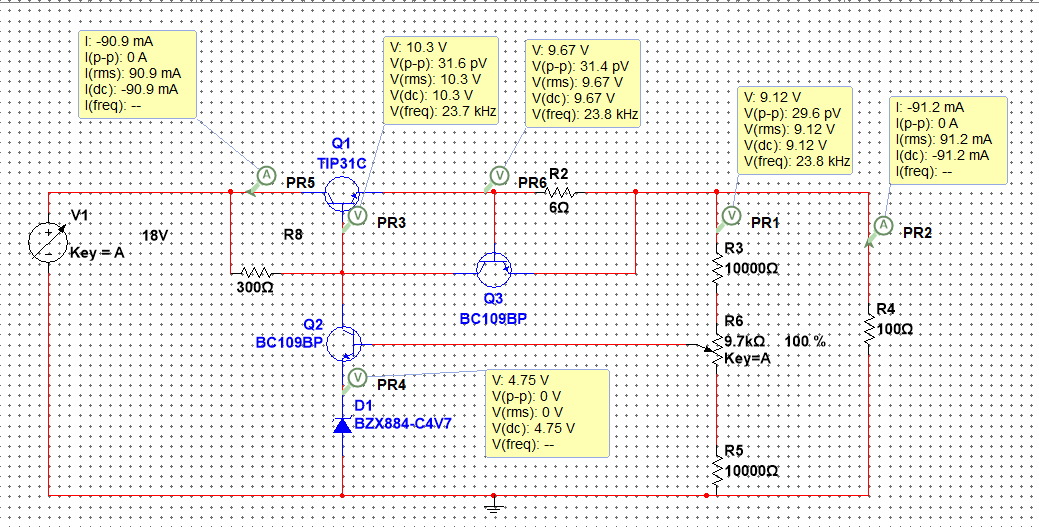
\includegraphics[width=0.7\textwidth]{during current limiting.png}
    \caption*{Current limiting feature}
\end{figure*}

%\newpage
\section{Measurements}

\begin{figure*}[h!]
\centering
    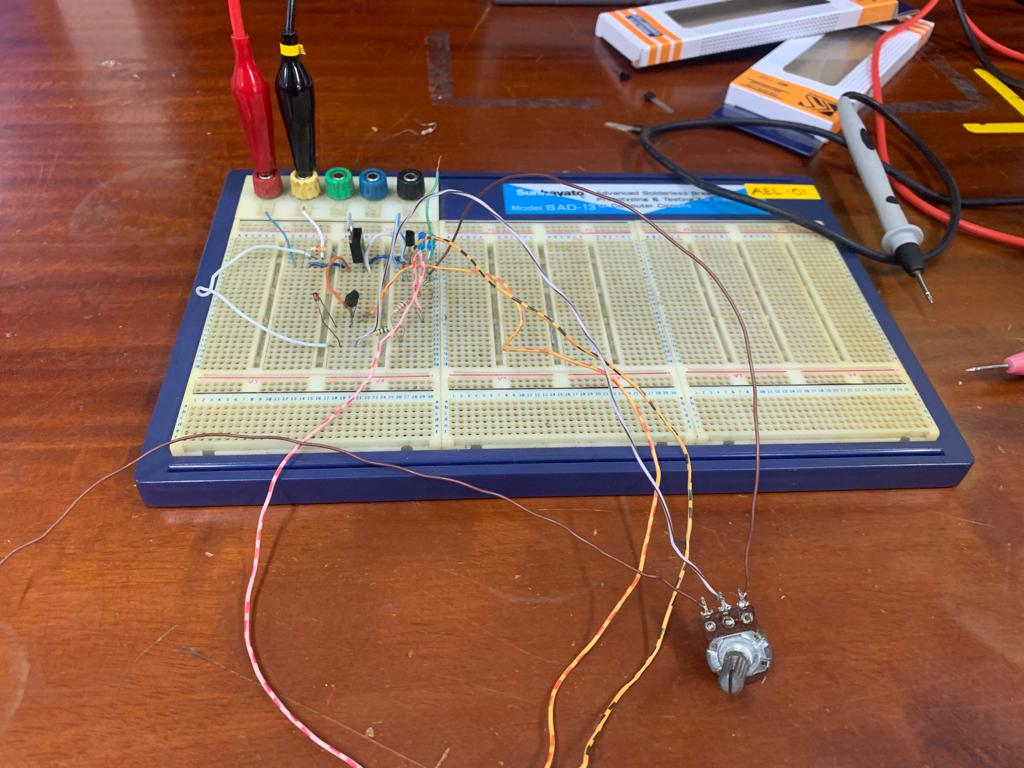
\includegraphics[width=0.4\textwidth]{our cct.jpg}
    %\caption*{Current limiting feature}
\end{figure*}

\newpage
\subsection{Line Variance}

\begin{figure*}[h!]
\centering
    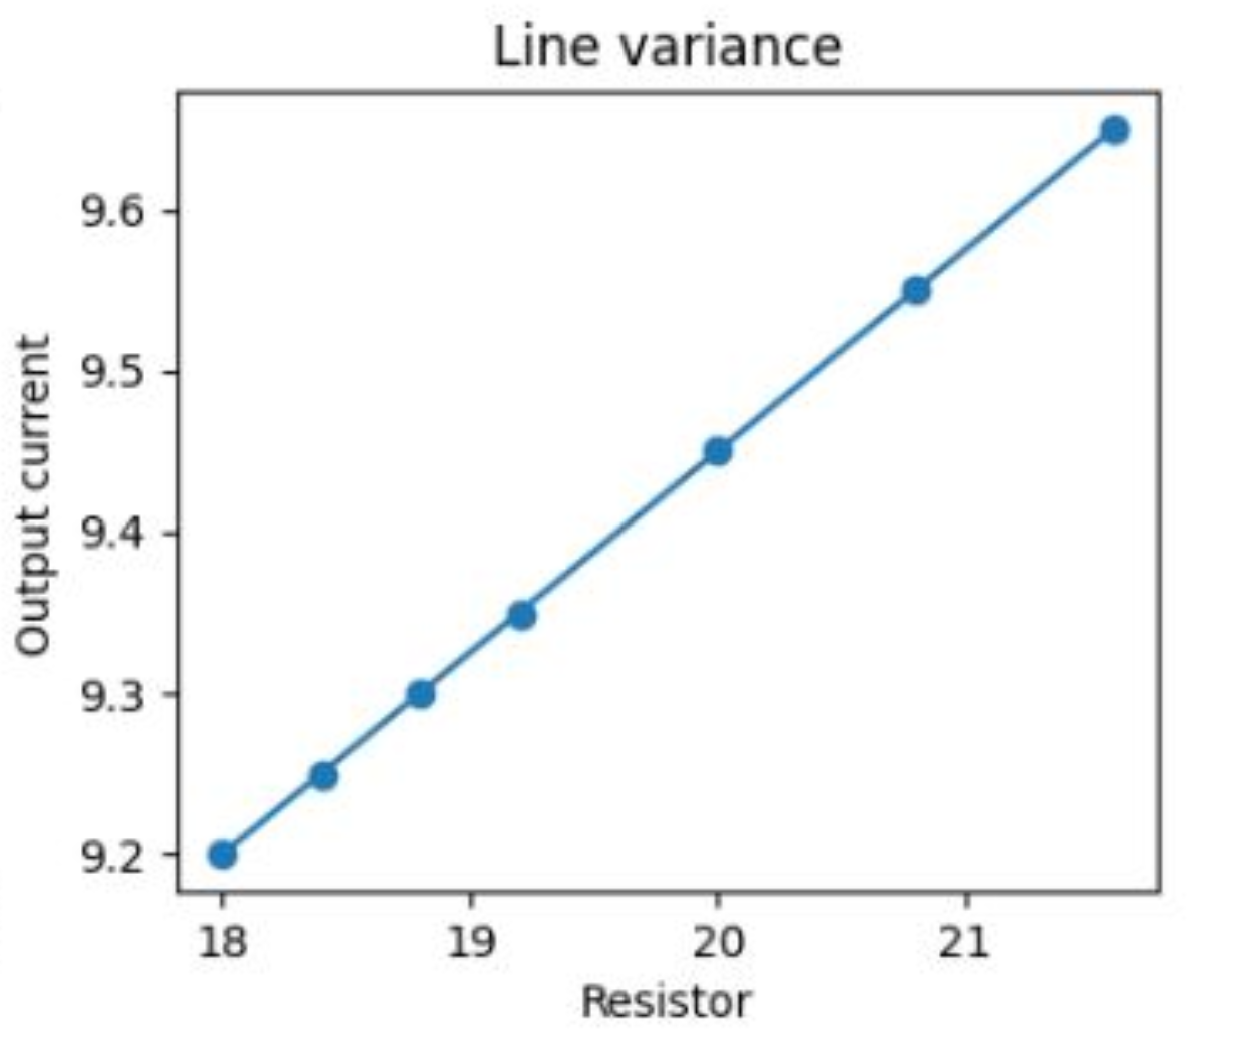
\includegraphics[width=0.4\textwidth]{Line Variance.png}
\end{figure*}

\subsection{Current Limiting Value}

\begin{equation*}
I_L \cdot r = 0.6
\end{equation*}
\begin{equation*}
(0.1) \cdot r = 0.6
\end{equation*}
\begin{equation*}
r = 6\,\Omega
\end{equation*}

We obtained a current of 130 mA during the current limiting process, which should be duly noted. The reason for this was the unavailability of a $1\,\Omega$ resistor, compelling us to utilize a 5-ohm resistor instead.

\begin{figure*}[h!]
\centering
    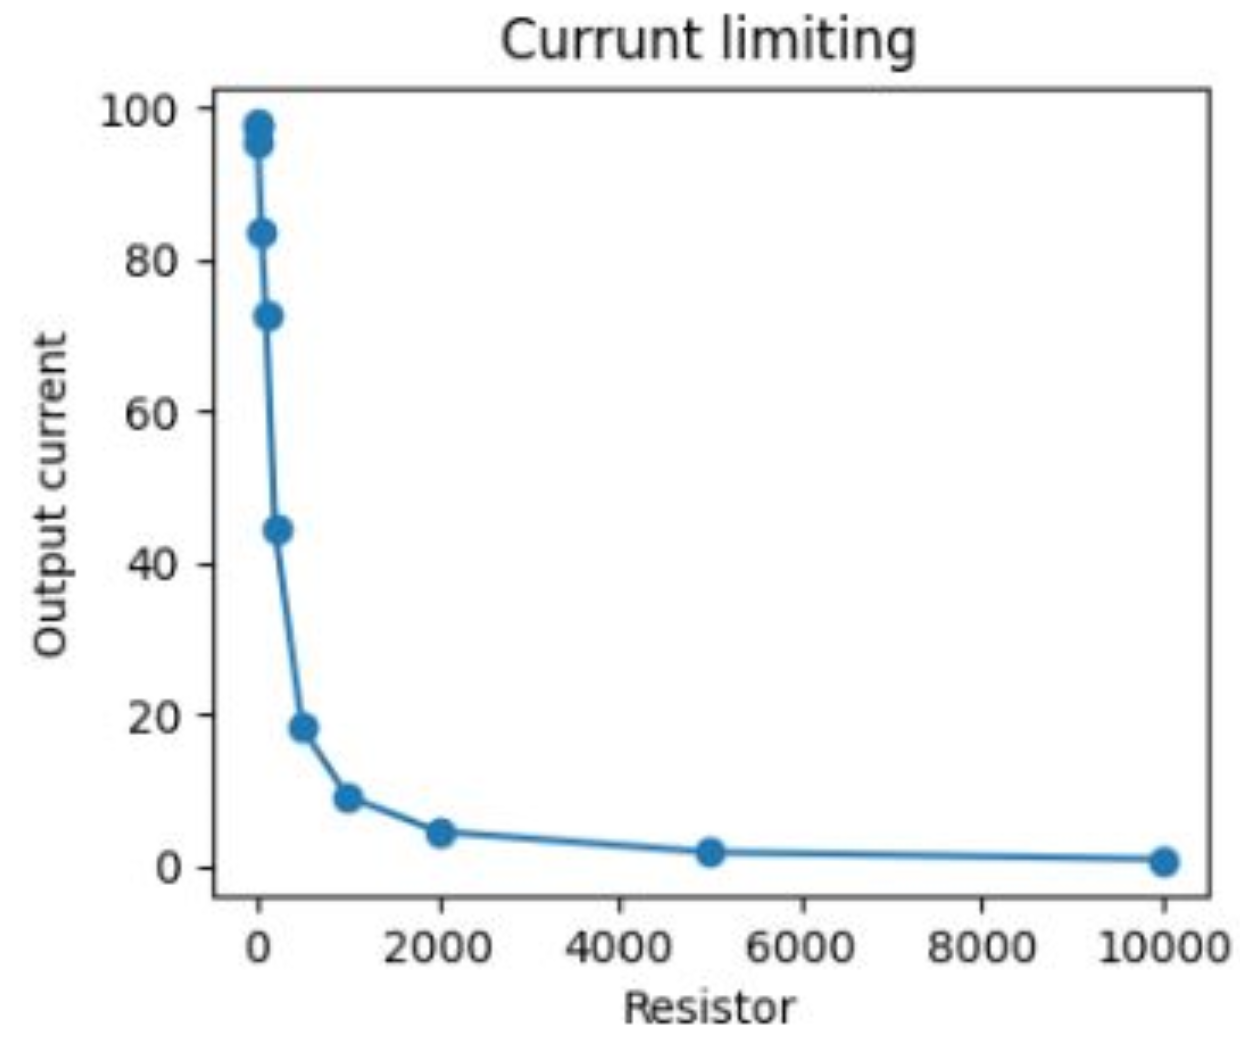
\includegraphics[width=0.4\textwidth]{Current Limiting.png}
\end{figure*}

\begin{figure*}[h!]
\centering
    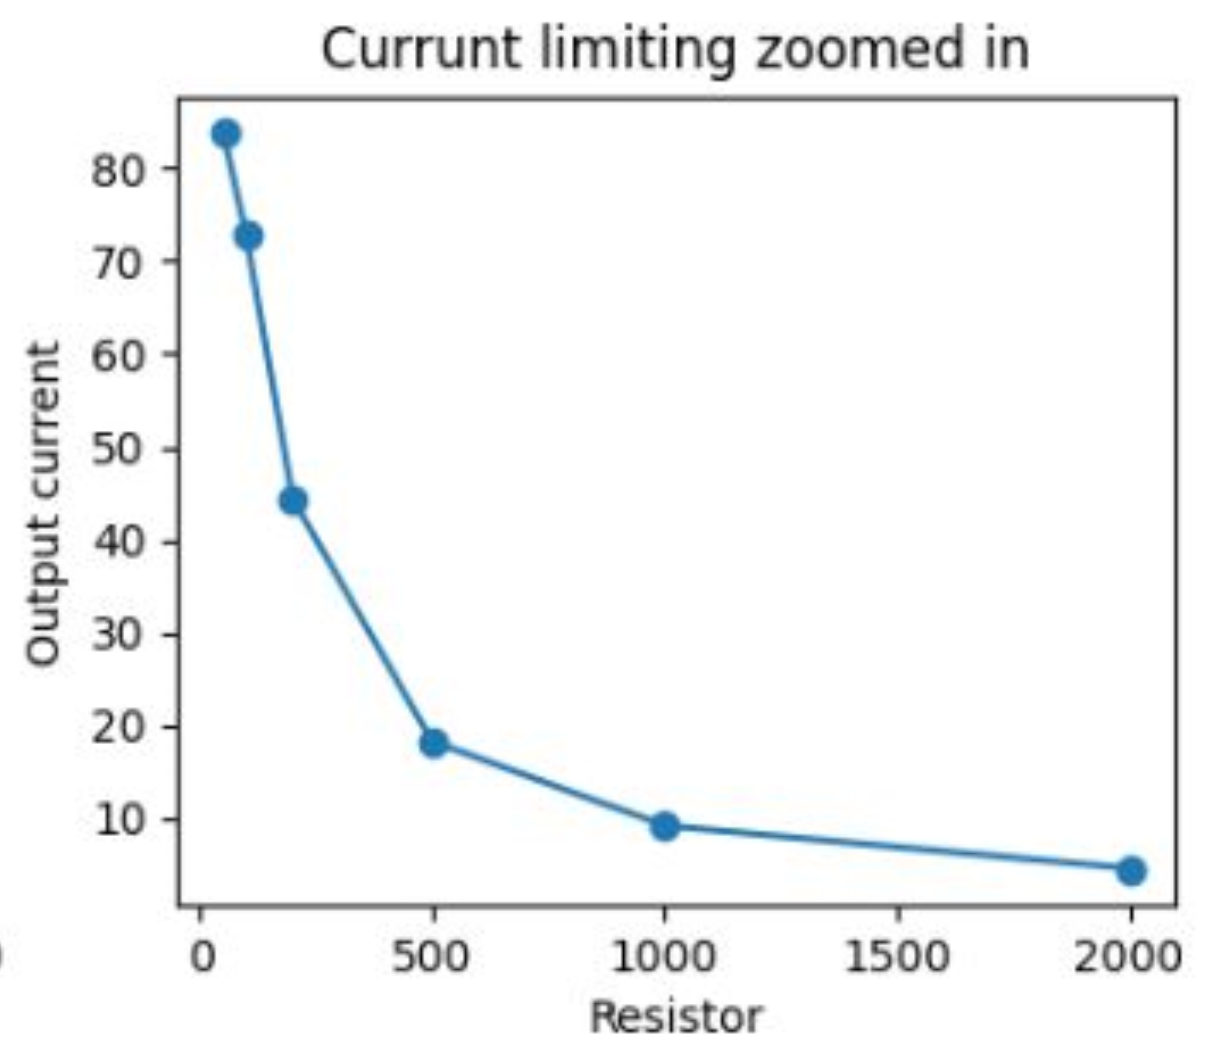
\includegraphics[width=0.4\textwidth]{Current Limiting Zoomed.png}
\end{figure*}

\newpage
\subsection{Load Regulation}

\begin{figure*}[h!]
\centering
    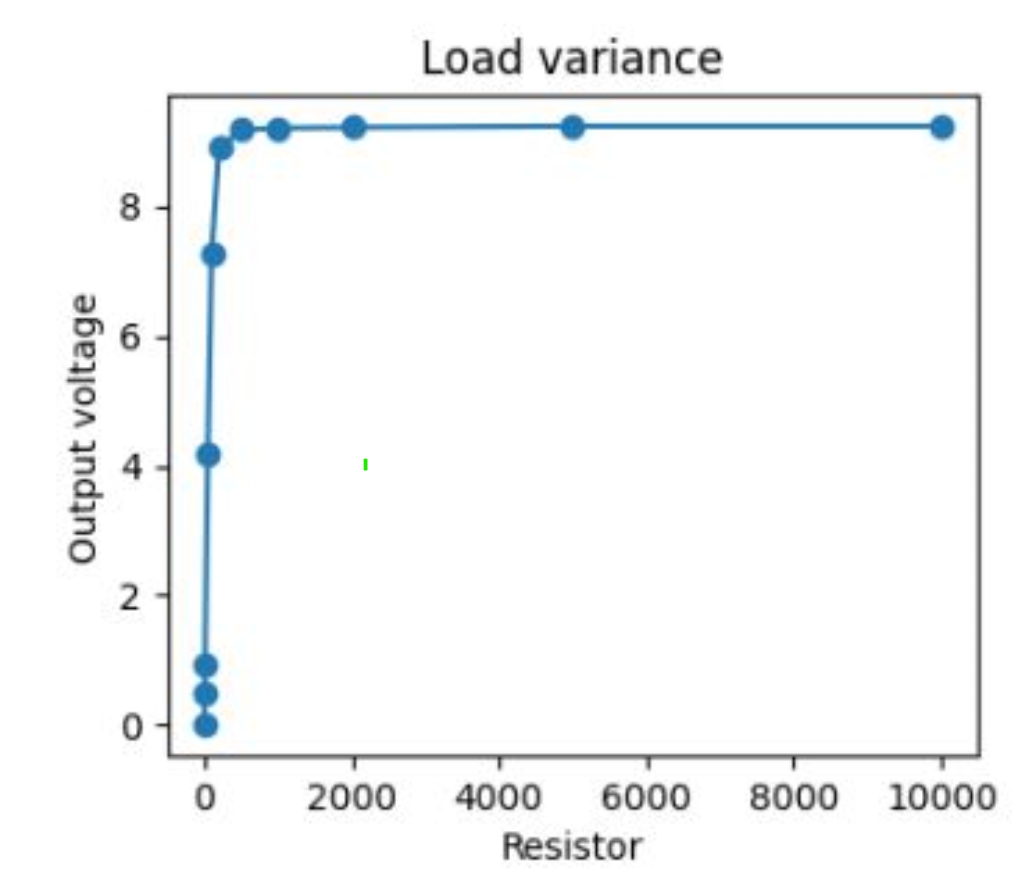
\includegraphics[width=0.4\textwidth]{Load Variance.png}
    %\caption*{Load variance}
\end{figure*}

\begin{figure*}[h!]
\centering
    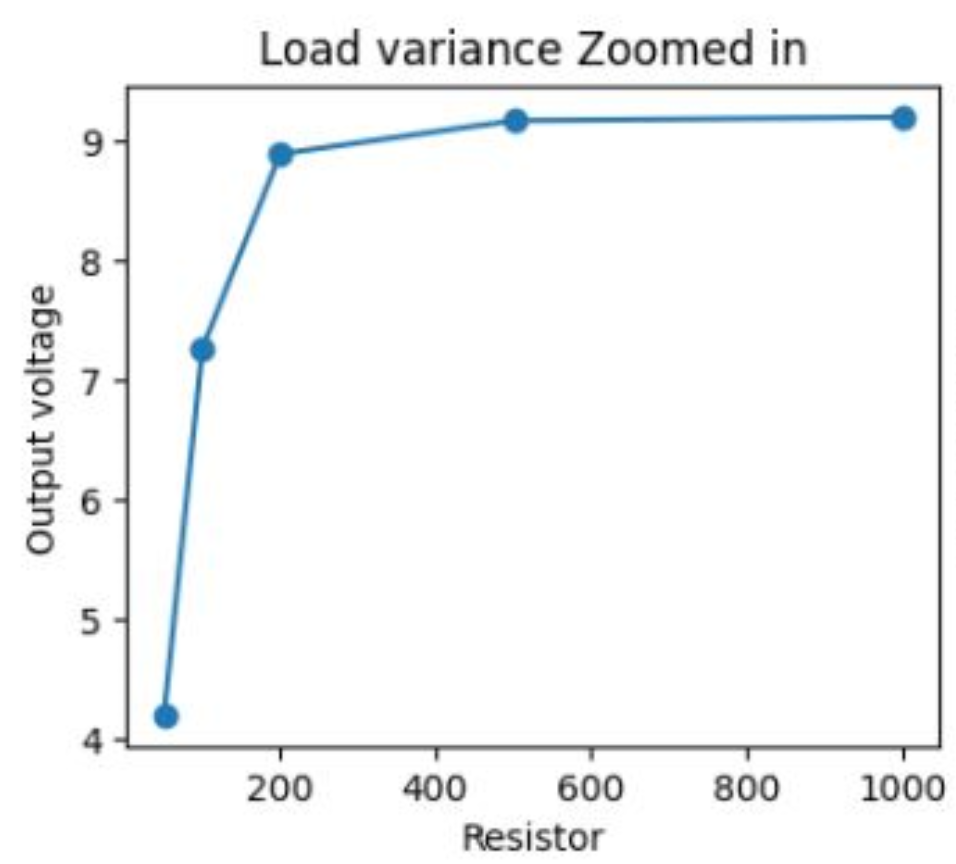
\includegraphics[width=0.4\textwidth]{Load Variance Zoomed.png}
    %\caption*{Load variance zoomed in}
\end{figure*}

\end{document}
